\section{Second Step : Fluxional Compiler} \label{chapter5:flx}

% The previous section presented a compiler to identify and extract the underlying pipeline in a Javascript application.
% However, the stages doesn't enforce the isolation required for parallel execution.
% Moreover, the Dues that constitues the stages of this pipeline only parts of the pipeline are identified, 

The second contribution of this thesis is the equivalence between a global memory abstraction and a distributed memory.
% between a memory shared among all the operations and independent memory for each operation in a pipeline.
It tackles the problems arising from the replacement of the global memory synchronizations with message passing.

This equivalence is implemented as a compiler, improving upon the previous one.
The compiler transforms a Javascript application into a network of independent parts communicating by message streams and executed in parallel.

Like the previous compiler, this compiler is organized into two main steps.
The first step is the identification of the rupture points between fluxions, addressed in section \ref{chapter5:flx:compiler}.
The second step is the isolation between the fluxions, addressed in section \ref{chapter5:flx:isolation}.
% The compiler, and the equivalence are described in section \ref{chapter5:flx:compiler}.
The compiler is tested on a real-case, to expose its limits in section \ref{chapter5:flx:evaluation}.
% Section \ref{chapter5:flx:evaluation} presents a real-case test of compilation, and expose the limits of this compiler.

% We named these parts \textit{fluxions}, by contraction between a flux and a function.
% Fluxions are executed in an execution model that assure parallelism and communications.

% We present an early version of this tool as a proof of concept for this compilation approach.
% Section \ref{chapter5:flx:model} describes the execution model that executes fluxions in parallel, and assure their communications.

\subsection{Fluxions Compiler} \label{chapter5:flx:compiler}

The source language for this transformation is of higher-order to allow the modularity required for productivity. 
Moreover, it is implemented as an event-loop to impose the developer to define the causality between asynchronous operations.
% Javascript is such a language and is often implemented on top of an event-loop, like in \textit{Node.js}.
The compiler transforms a \textit{Node.js} application into a fluxional application compliant with the execution model described in section \ref{chapter4:flx-model}.
The chain of compilation is described in figure \ref{fig:compilation}.

\begin{figure}
  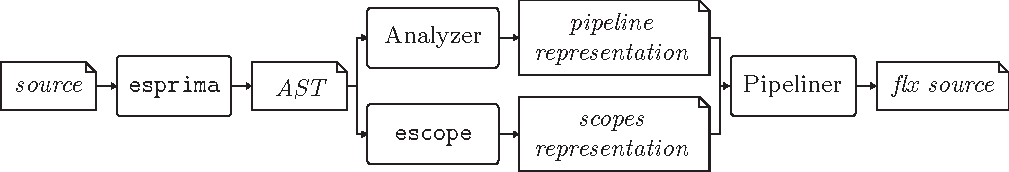
\includegraphics[width=\linewidth]{../resources/compiler-stream.pdf}
  \caption{Compilation chain}
  \label{fig:compilation}
\end{figure}

The compiler uses the \textit{estools}\ftnt{https://github.com/estools} suite to parse (\texttt{esprima}), analyze (\texttt{escope}), manipulate (\texttt{estraverse} and \texttt{esquery}) and generate (\texttt{escodegen}) source code from an Abstract Syntax Tree (AST).
It is tailored for -- but not limited to -- web applications using \textit{Express}\ftnt{http://expressjs.com/}, the most used \textit{Node.js} web framework.
The compiler extracts an AST from the source with \texttt{esprima}.
From this AST, the \textit{Analyzer} step identifies the rupture points between the different application parts. % and how they relate to form a pipeline.
This first step outputs a pipeline representation of the application.
% Section \ref{chapter5:flx-compiler:analyzer} explains this first compilation step.
In this pipeline representation, the stages are not yet independent and encapsulated into fluxions.
From the AST, \texttt{escope} produces a representation of the memory scopes.
The \textit{Pipeliner} step, explained in section \ref{chapter5:flx:isolation}, analyzes the pipeline representation and the scopes representation to distribute the shared memory into independent groups of fluxions.
% Section \ref{chapter5:flx-compiler:pipeliner} explains this second compilation step.

% \subsubsection{Analyzer step} \label{chapter5:flx-compiler:analyzer}

% The limit between two application parts is defined by a rupture point.
% The analyzer identifies the rupture points, and outputs a representation of the application in a pipeline form.
% Application parts are the stages, and rupture points are the message streams of this pipeline.

\subsubsection{Detection}

In \textit{Node.js}, I/O operations are asynchronous functions and indicate rupture points between two application parts.
Figure \ref{fig:basicrp} shows a code example of a rupture point with the illustration of the execution of the two application parts isolated into fluxions.
The two application parts are the caller of the asynchronous function call on one hand, and the callback provided to the asynchronous function call on the other hand.

\begin{figure}[h!]
  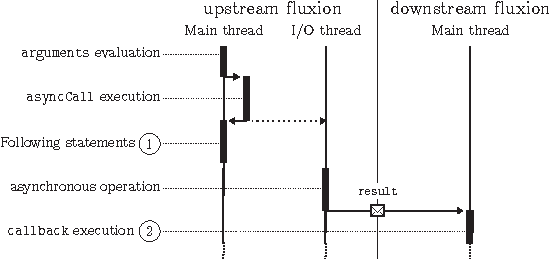
\includegraphics[width=0.8\linewidth]{../resources/basicrp.pdf}
  \begin{code}
asyncCall(arguments, function callback(result){ //@\circled{2}@ });
// Following statements //@\circled{1}@
  \end{code}
  \caption{Rupture point interface}
  \label{fig:basicrp}
\end{figure}

Similarly as in the Due compiler, the detection of asynchronous callees is done by the developer. 
It uses a list of common asynchronous callees, like the \texttt{express} and file system methods.
This list can be augmented to match asynchronous callees individually for any application.
To identify the callee, the analyzer walks the AST to find a call expression matching this list.

After the identification of the callee, the callback needs to be identified as well to be encapsulated in the downstream fluxion.
For each asynchronous call detected, the compiler tests if one of the arguments is of type \texttt{function}.
The callback functions declared \textit{in situ} are trivially detected in the AST.
The compiler discard callbacks not declared \textit{in situ}, to avoid altering the semantic by moving or modifying their definitions.
% For variable identifiers, and other expressions, the analyzer tries to detect their type.
% The analyzer walks back the AST to track their assignations and modifications, so as to determine their last value.





% \comment{TODO insert this}
% We developed the compiler core in node.js Javascript.
% There already exist sets of tools for manipulating code in Javascript.
% We used the Esprima suite of tools.
\subsection{Fluxions Isolation} \label{chapter5:flx:isolation}

A rupture point eventually breaks the chain of scopes between the upstream and downstream fluxion.
The closure in the downstream fluxion cannot access the scope in the upstream fluxion as expected.
The pipeliner step replaces the need for this closure, allowing application parts to rely only on independent memory stores and message passing.
It determines the distribution using the scope representation, which represents the variables' dependencies between application parts.
Depending on this representation, the compiler can replace the broken closures in three different ways.
We present these three alternatives in figure \ref{fig:states}.

\begin{figure}[h!]
  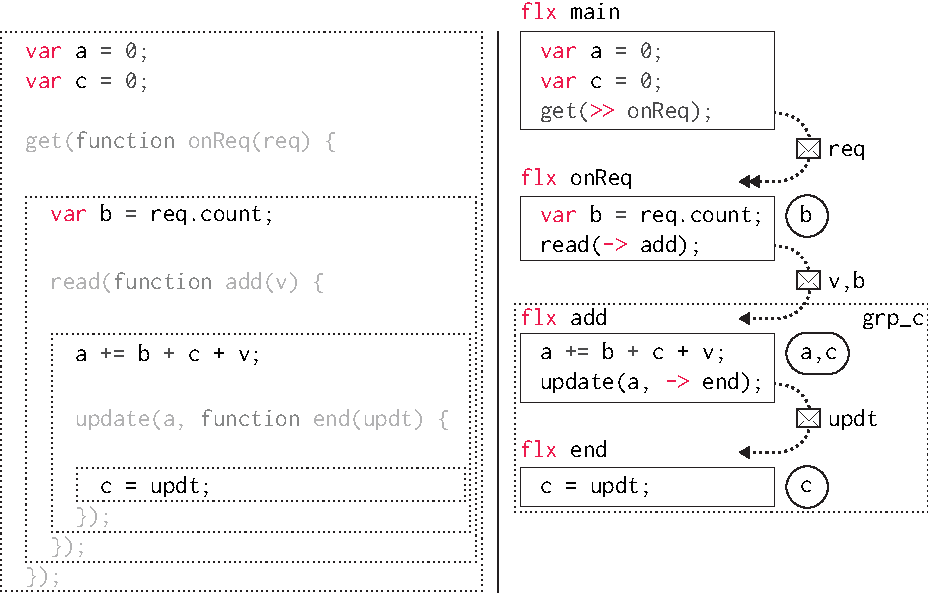
\includegraphics[width=\linewidth]{../resources/states.pdf}
  \caption{Variable management from Javascript to the high-level fluxionnal language}
  \label{fig:states}
\end{figure}

\paragraph{Scope}
If a variable is modified inside only one application part in the current \textit{post} chain, then the pipeliner adds it to the context of its fluxion.

In figure \ref{fig:states}, the variable \texttt{a} is updated in the function \texttt{add}.
The pipeliner step stores this variable in the context of the fluxion \texttt{add}.

\paragraph{Stream}
If a modified variable is read by downstream application parts, then the pipeliner makes the upstream fluxion add this variable to the message stream to be sent to the downstream fluxions.
It is impossible to send variables to upstream flux\-ions, without causing inconsistencies.
If the fluxion retro propagates the variable for an upstream fluxion to read, the upstream fluxion might use the old version while the new version is on its way.

In figure \ref{fig:states}, the variable \texttt{b} is set in the function \texttt{onReq}, and read in the function \texttt{add}.
The pipeliner step makes the fluxion \texttt{onReq} send the updated variable \texttt{b}, in addition to the variable \texttt{v}, in the message sent to the fluxion \texttt{add}.

Exceptionally, if a variable is defined inside a \textit{post} chain, like \texttt{b}, then this variable can be streamed inside this \textit{post} chain without restriction on the order of modification and read.
Indeed, the execution of the upstream fluxion for the current \textit{post} chain is assured to end before the execution of the downstream fluxion.
Therefore, no reading of the variable by the upstream fluxion happens after the modification by the downstream fluxion.

\paragraph{Share}
If a variable is needed for modification by several application parts, or is read by an upstream application part, then it needs to be synchronized between the fluxions.
To respect the semantics of the source application, we cannot tolerate inconsistencies.
Therefore, the pipeliner groups all the fluxions sharing this variable with the same tag.
And it adds this variable to the contexts of each fluxions.

In figure \ref{fig:states}, the variable \texttt{c} is set in the function \texttt{end}, and read in the function \texttt{add}.
As the fluxion \texttt{add} is upstream of \texttt{end}, the pipeliner step groups the fluxion \texttt{add} and \texttt{end} with the tag \texttt{grp\_c} to allow the two fluxions to share this variable.
\section{Overall Evaluation} \label{chapter6:evaluation}

The equivalence presented in chapter \ref{chapter4} is implemented in a the fluxional compiler, presented in section \ref{chapter5:flx}.
This implementation is evaluated against the criteria presented in chapter \ref{chapter3}, Productivity, Efficiency and Adoption.

\subsection{Trading Productivity for Efficiency}

% \subsubsection{Productivity}

The equivalence intends to disrupt as less as possible the way developer build web applications.
The goal is to avoid degrading the productivity, hence the adoption, of the proposed platform.
% The source language, Javascript, is left intact, except for the forbidden statements \texttt{with} and \texttt{eval}.
% These statements are already forbidden by some good practice guides \cite{Crockford2008}.
Therefore, the productivity is intended to be the same as the original event-driven platform.

However, in the current state, the compiler implementation is unable to operate the transformation without an external help.
The static analysis is unable to correctly detect the aliasing of the memory in Javascript.
It avoids developers to use Higher-Order Programming, hence impacts composition.
This limitation avoids to improve the current trade-off of productivity for efficiency, as illustrated in table \ref{tab:proposition-productivity}.
Indeed, to gain efficiency, developers need to commit efforts to indicate the stages of the pipeline, and assure their dependency.

% \TablePropositionProductivity{tab:proposition-productivity}

The manual transformation process yields a distributed application, similarly as the other efficient platforms.
And the chapter \ref{chapter3} showed that such applications achieve very good performance efficiency.
But the productivity limitation remains.
It avoids the current implementation to propose a satisfying compromise between productivity and efficiency.
So, the current implementation actually trades productivity for efficiency, similarly to many platform in the state of the art. % , as illustrated in table \ref{tab:proposition-efficiency}.
The perspectives to overcome this limitation are addressed later in section \ref{chapter5:evaluation:perspective}.
% \TablePropositionEfficiency{tab:proposition-efficiency}


% It doesn't make any sense to evaluate an application, as the transformation would not reflect the compilation process, but the manual transformation process.

% If the runtime memory analysis is solid enough to detect correctly the aliasing of the memory, then it will be able to help the development team transitioning from productivity to efficiency, which is the response of this thesis to the problematic.

\subsection{Adoption}

As observed in the chapter \ref{chapter3}, trading productivity for efficiency drastically reduces adoption.
Because the current implementation presents the same limitation than the efficient platforms, its adoption is not expected to be different. %, as illustrated in table \ref{tab:proposition-adoption}.

Yet, both productivity and efficiency are required for the platform to be adopted by new developers as well as large businesses.
Only at this condition, will it reinforce the loop between community and industry.
So the current implementation is not expected to be widely adopted, as presented in the table \ref{tab:proposition-summary}.

\TablePropositionSummary{tab:proposition-summary}
% \TablePropositionAdoption{tab:proposition-adoption}

% It was briefly tested during the development of the grumpy application, presented in chapter \ref{chapter4}, section \ref{chapter4:execution-models:examples}.

The limitation of static analysis avoids the equivalence to be fully implemented to address the problematic.
Hence, this evaluation holds only on the implementation, and not on the equivalence.


When saying that \textit{it is a mistake to attempt high concurrency without help from the compiler}, R. von Behren \textit{et al.} \cite{Behren2003} implies that the language alone cannot achieve high concurrency.
It is necessary to rely on additional tools, such as a compiler to reach the best compromise between productivity and efficiency.
The evaluation of this thesis concludes that static analysis is unable to reach this compromise for the current multi-paradigm languages using higher-order programming.
% Before dropping all higher-order languages for the sake of efficiency,
Yet, there exist alternatives to static analysis to reach this compromise.
The next paragraph presents some interesting perspectives of this work to further address this problematic.

% In the contribution of this thesis, the two main difficulties, identifying stages and detecting memory dependencies, are due to the dynamic nature of Javascript.
% A perspective to overcome these limitation is to implement the transformation, not as a compiler, but as a runtime.
% Indeed, at runtime, all the dynamic behavior are resolved, and the analysis can be much more precise, and less speculative.

% \subsection{Fluxionnal Runtime} 

% \section{Perspectives}

% Javascript is a highly dynamic languages.